\documentclass[aspectratio=169]{beamer}
 
\usetheme[sectionpage=none, subsectionpage=none, progressbar=none]{metropolis}           % Use metropolis theme
 
  \usepackage{outlines}
  \usepackage{caption}
  \usepackage{appendixnumberbeamer}
  \usepackage{booktabs}
  \usepackage{tcolorbox}
  \usepackage{tabularx}
  \usepackage[export]{adjustbox}[2011/08/13]
  \usepackage{bm}

\newcolumntype{R}{>{\raggedleft\arraybackslash}X} 
  
 \setbeamertemplate{footline}[frame number]{}

\setbeamertemplate{footline}{% 
  \hfill% 
  \usebeamercolor[fg]{page number in head/foot}% 
  \usebeamerfont{page number in head/foot}% 
  \insertframenumber%
  %\,/\,\inserttotalframenumber
  \kern1em\vskip2pt% 
}

\makeatletter
\setbeamertemplate{headline}{%
  \begin{beamercolorbox}[colsep=1.5pt]{upper separation line head}
  \end{beamercolorbox}
  \begin{beamercolorbox}{section in head/foot}
    \vskip2pt\insertnavigation{\paperwidth}\vskip2pt
  \end{beamercolorbox}%
  \begin{beamercolorbox}[colsep=1.5pt]{lower separation line head}
  \end{beamercolorbox}
}
\let\@@magyar@captionfix\relax % IMPORTANT: This is a workaround to fix a random eror with the 2018 installation
\makeatother

\usepackage{xcolor} 
\listfiles

\setbeamercolor{section in head/foot}{fg=normal text.bg, bg=structure.fg}

    \usepackage{smartdiagram}
    \usepackage{tikz}
\usetikzlibrary{shapes.geometric, arrows}
\tikzstyle{startstop} = [rectangle, rounded corners, minimum width=3cm, minimum height=1cm,text centered, draw=black, fill=red!30]
\tikzstyle{io} = [trapezium, trapezium left angle=70, trapezium right angle=110, minimum width=3cm, minimum height=1cm, text centered, draw=black, fill=blue!30]
\tikzstyle{process} = [rectangle, minimum width=3cm, minimum height=1cm, text centered, draw=black, fill=orange!30]
\tikzstyle{decision} = [diamond, minimum width=3cm, minimum height=1cm, text centered, draw=black, fill=green!30]

\title{Gov 2006: Formal Political Theory II \\
Section 3}
\date{\today}
\author{ \textbf{Sophie Hill}}


\begin{document}
  \maketitle
  

%%%%%%%%%%%%%%%%%%%%%%%%%%%%%%%%%%%%%%%%%%
\begin{frame}{Agenda}



\begin{itemize}
\setlength \itemsep{0.5em}
\item Probabilistic voting: mini-review

\item Models of spending on public goods (Downs, Bergstrom 
\& Goodman, Meltzer \& Richard, and beyond!)

\item Brainstorming final paper ideas!


\end{itemize}

\end{frame}
%%%%%%%%%%%%%%%%%%%%%%%%%%%%%%%%%%%%%%%%%%
\begin{frame}{Probabilistic voting: mini-review}

\begin{outline}
\setlength \itemsep{0.5em}
\1 You should now be relatively familiar with the set-up of the probabilistic voting model...
\pause
\1 In this model, there are two random shocks: an \alert{individual} shock $\sigma_i \sim U \left[ -\frac{1}{2 \phi}, \frac{1}{2 \phi} \right] $ and a \alert{common} shock $\delta \sim U \left[ -\frac{1}{2 \psi}, \frac{1}{2 \psi} \right] $
\pause
\1 What is the substantive interpretation of the following terms?
\pause 
\2 $\sigma_i$ \pause = \alert{individual ideology parameter}
\2 $\delta$ \pause = \alert{incumbent popularity shock}
\2 $\phi$ \pause = \alert{voter sensitivity to policy}

\1 A common extension to this model is to let the ideology parameter have a group-specific distribution, $\sigma_{Ji}$. We can then vary group-level ideology (i.e. $\mathbb{E}[\sigma_{Ji}] \neq \mathbb{E}[\sigma_{Ki}] $) and sensitivity to policy (i.e. $\phi_J \neq \phi_K$).

\end{outline}

\end{frame}
%%%%%%%%%%%%%%%%%%%%%%%%%%%%%%%%%%%%%%%%%%
\begin{frame}{Probabilistic voting: mini-review}

Higher density = more sensitive to policy = ``swing voters''
\centering
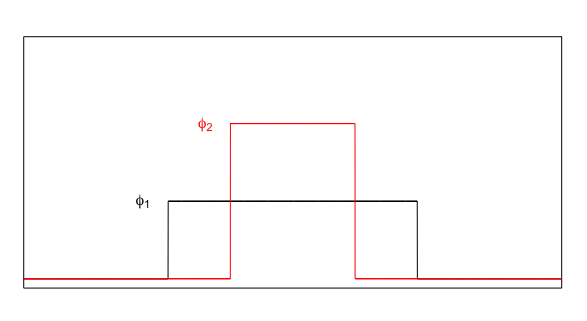
\includegraphics[width=0.85\textwidth]{pdf.png}

\end{frame}

%%%%%%%%%%%%%%%%%%%%%%%%%%%%%%%%%%%%%%%%%%
\begin{frame}{Probabilistic voting: mini-review}

Shift midpoint of $\sigma$ = ideological bias = ``partisans''
\centering
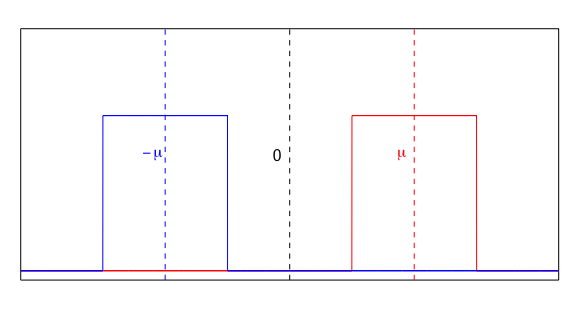
\includegraphics[width=0.85\textwidth]{pdf2.png}

\end{frame}

%%%%%%%%%%%%%%%%%%%%%%%%%%%%%%%%%%%%%%%%%%
\begin{frame}{Models of spending on public goods}

\Large 

The papers last week were speaking to two central puzzles of democratic distributive politics:

\begin{itemize}
\item Why is the size of government growing over time?

\item How does ``rational ignorance'' affect provision of public goods?
\end{itemize}


\end{frame}
%%%%%%%%%%%%%%%%%%%%%%%%%%%%%%%%%%%%%%%%%%
\begin{frame}{Models of spending on public goods}


\centering
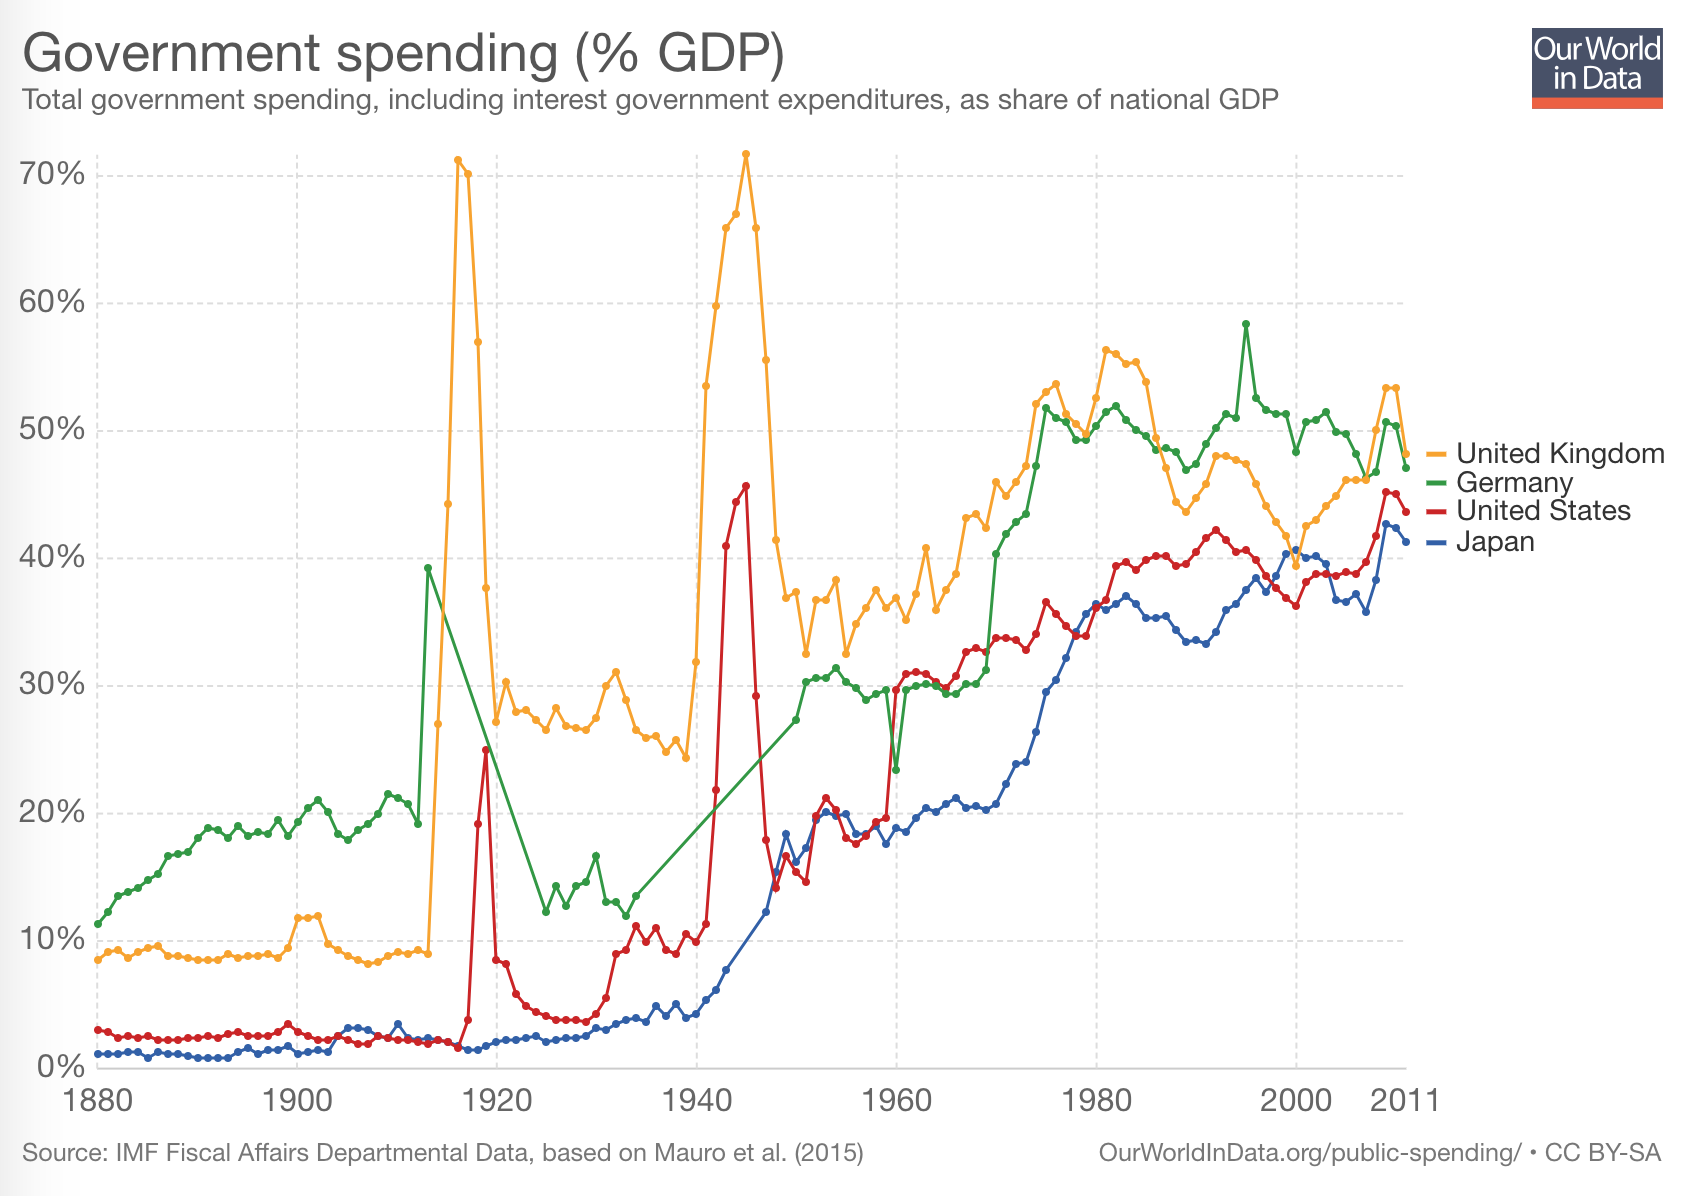
\includegraphics[width=0.70\textwidth]{gov_spending.png}

\end{frame}

%%%%%%%%%%%%%%%%%%%%%%%%%%%%%%%%%%%%%%%%%%
\begin{frame}{Models of spending on public goods}


\centering
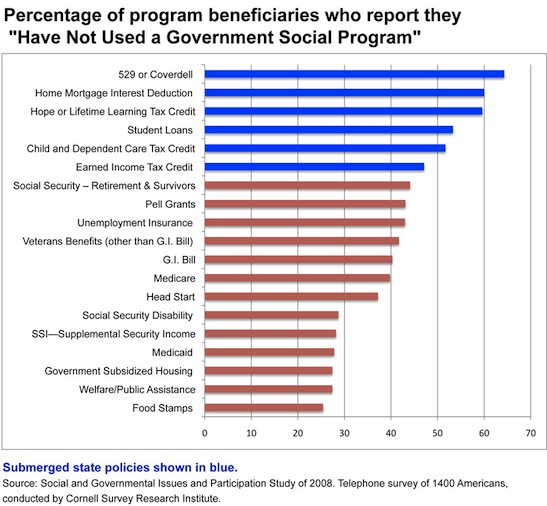
\includegraphics[width=0.50\textwidth]{mettler.png}

\end{frame}
%%%%%%%%%%%%%%%%%%%%%%%%%%%%%%%%%%%%%%%%%%
\begin{frame}{Models of spending on public goods}

\Large
These are big motivating puzzles... \pause but let's start with a simpler question: how should we model citizen preferences over public goods?

\end{frame}

%%%%%%%%%%%%%%%%%%%%%%%%%%%%%%%%%%%%%%%%%%
\begin{frame}{Bergstrom \& Goodman, 1973}

\begin{itemize}
\item Individual utility is a function of private and public goods: $U_i = f(X_i, Z_i)$ 
\pause
\item An individual derives utility from the total public good based on the population $n$ and a ``crowding parameter'' $\gamma$: $Z_i = \frac{Z}{n^\gamma}$
\pause
\item $\gamma = 1 \rightarrow$ purely private good
\pause
\item $\gamma = 0 \rightarrow$ purely public good
\pause
\item Individual maximizes utility subject to her budget contraint $X_i + \tau_i q n^\gamma Z_i \leq Y_i$, where $q$ is the unit cost of the public good and $\tau_i$ is $i$'s tax share

\end{itemize}


\end{frame}

%%%%%%%%%%%%%%%%%%%%%%%%%%%%%%%%%%%%%%%%%%
\begin{frame}{Bergstrom \& Goodman, 1973}

\begin{itemize}
\item Assume constant income and price elasticities for the public good $\delta$ and $\epsilon$
\pause
\item Then the demand function for $Z_i$ has the form: $c[ \tau_i q n^\gamma ]^\delta Y_i^\epsilon$
\pause
\item So the demand for $Z$ is: $n^\gamma c[ \tau_i q n^\gamma ]^\delta Y_i^\epsilon = c q^\delta \tau_i^\delta Y_i^\epsilon n^{\gamma (1 + \delta)}$
\pause
\item We can estimate these elasticities by fitting this regression model: $ \log E = c + \alpha \log n + \delta log \hat{\tau} + \epsilon \log \hat{Y} + \sum_{i=1}^k \beta_i X_i$
\pause
\item where $E$ = expenditures, $n$ = \# of households, $\hat{\tau}$ = tax share of citizen with median income, $\hat{Y} $ = median income, and the $X_i$'s are municipality socio-economic controls.

\end{itemize}


\end{frame}
%%%%%%%%%%%%%%%%%%%%%%%%%%%%%%%%%%%%%%%%%%
\begin{frame}{Bergstrom \& Goodman, 1973}

\begin{itemize}
\item How does demand vary with income?
\pause
\item Compute the total derivative: $ \frac{\mathop{dD}}{\mathop{dY}} = \frac{ \partial D}{ \partial Y } + \left( \frac{ \partial D }{ \partial \tau} \right) \left( \frac{ \partial \tau}{ \partial Y} \right) $
\pause 
\item In elasticity form: $ \left( \frac{Y}{D} \right) \left( \frac{ d D}{d Y } \right) = \epsilon + \delta \eta$
\pause 
\item $\epsilon$ = income elasticity of demand; $\delta$ = price elasticity of demand; $\eta$ = elasticity of tax share w.r.t income
\pause 
\item If $\epsilon + \delta \eta > 0$ for all $Y$, then individual demand for public goods is \textit{increasing} in income (and \textit{vice versa})
\pause 
\item It is also possible that the sign of $\epsilon + \delta \xi$ varies across values of $Y$, in which case the relationship is non-monotonic

\end{itemize}


\end{frame}

%%%%%%%%%%%%%%%%%%%%%%%%%%%%%%%%%%%%%%%%%%
\begin{frame}{Bergstrom \& Goodman, 1973}

\begin{itemize}
\item We can estimate $\epsilon$ and $\delta$ directly from the regression. What about $\xi$?
\pause 
\item Approximate it with commonly accepted estimates of income elasticity of demand for housing $\approx$ 1 - 1.3
\pause 
\item Almost all the estimates of $\epsilon$ are \textit{greater} than $-(1.3) \delta$
\pause
\item Hence we seem to be in a world where $\epsilon + \delta \xi > 0$, i.e. demand for public goods \textit{rises} with income
\end{itemize}

\begin{tcolorbox} \alert{Question}: How can we reconcile this with Meltzer-Richard? Is there something about this empirical context that doesn't fit the M-R model?
\end{tcolorbox}


\end{frame}

%%%%%%%%%%%%%%%%%%%%%%%%%%%%%%%%%%%%%%%%%%
\begin{frame}{U.S. state \& local taxes}


\centering
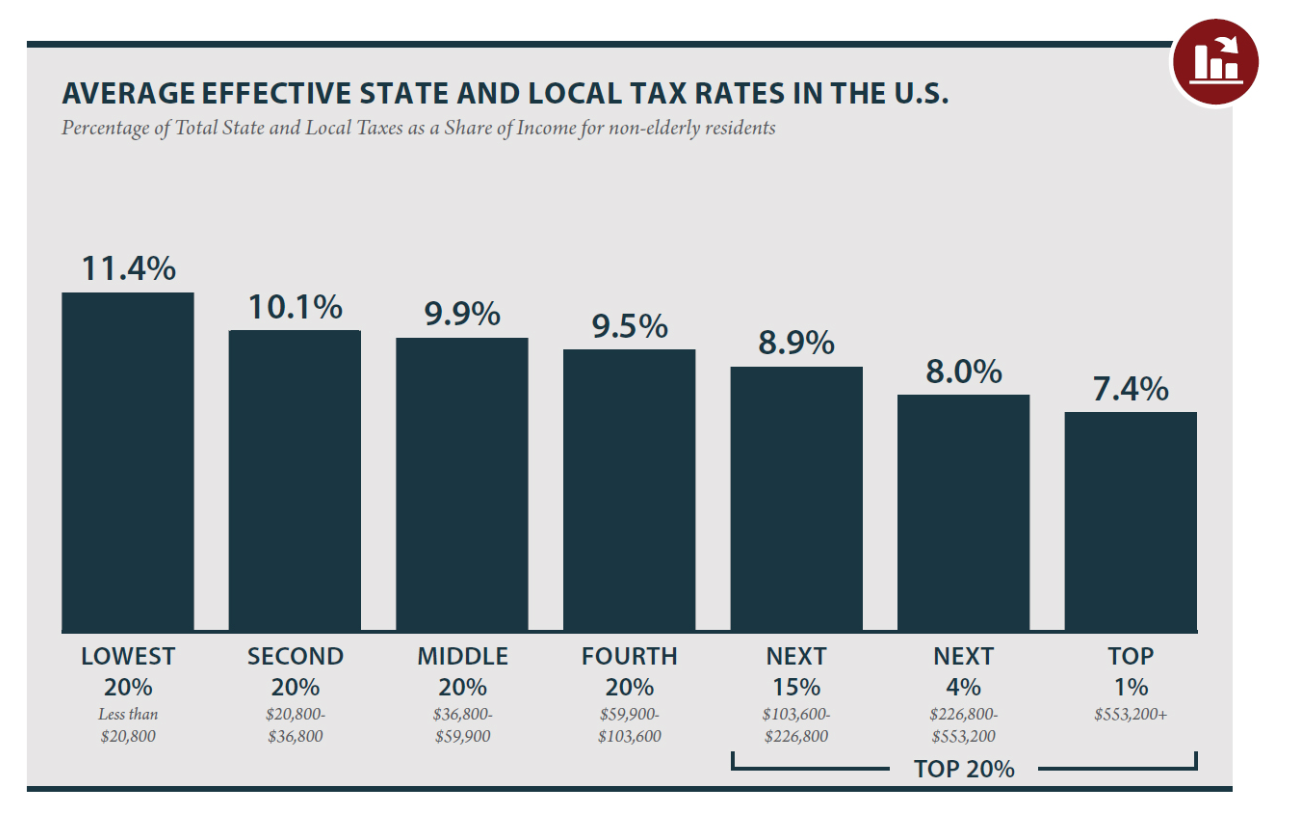
\includegraphics[width=0.8\textwidth]{local_taxes.png}

\end{frame}
%%%%%%%%%%%%%%%%%%%%%%%%%%%%%%%%%%%%%%%%%%
\begin{frame}{Meltzer-Richard, in one chart!}


\centering
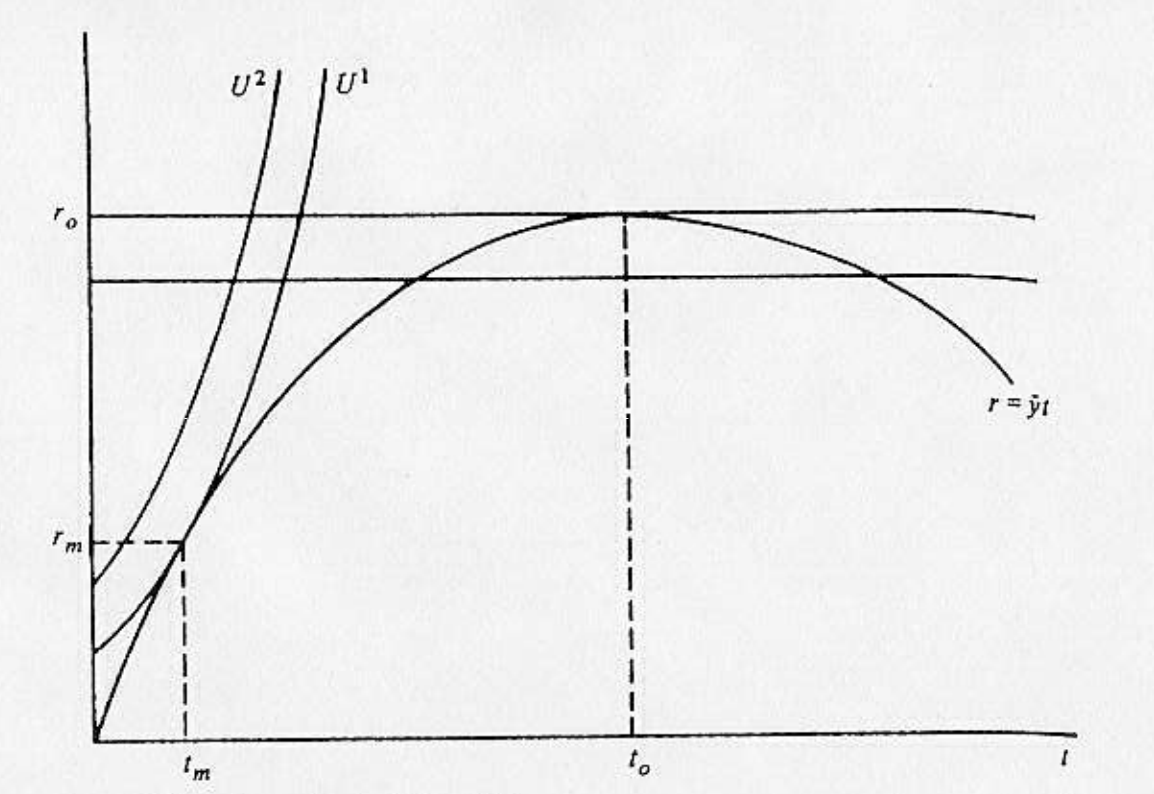
\includegraphics[width=0.7\textwidth]{mr.png}

\end{frame}
%%%%%%%%%%%%%%%%%%%%%%%%%%%%%%%%%%%%%%%%%%
\begin{frame}{Downs, 1960}

Several key assumptions:
\begin{enumerate}
\item Voters are \alert{rationally ignorant}
\pause 
\item Voters are more aware of the costs (i.e. the taxes they pay) than the benefits (which may be geographically or temporally remote) of public spending
\pause 
\item Politicians determine public spending solely to win votes
\end{enumerate}

\pause

Thus, electoral competition puts downward pressure on public spending -- it is smaller than it would be if voters were fully informed.

\pause

\begin{tcolorbox}
Questions: Are voters rationally ignorant, or genuinely misinformed? Is (3) plausible? Can we reconcile this argument with the empirical fact of growing government budgets?
\end{tcolorbox}

\end{frame}
%%%%%%%%%%%%%%%%%%%%%%%%%%%%%%%%%%%%%%%%%%
\begin{frame}{Downs, 1960}


\centering
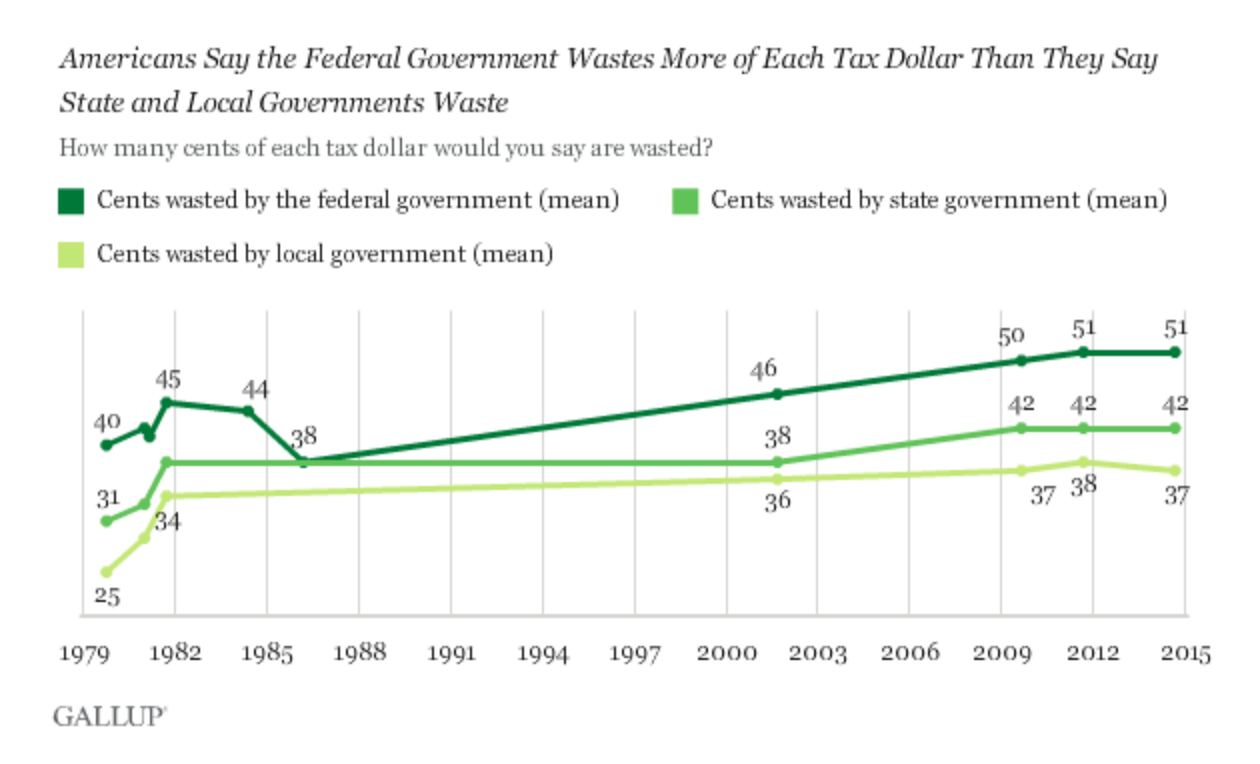
\includegraphics[width=0.8\textwidth]{gallup.png}

\end{frame}
%%%%%%%%%%%%%%%%%%%%%%%%%%%%%%%%%%%%%%%%%%
\begin{frame}{Extensions of M-R}

\begin{enumerate}

\item Public spending is about \alert{insurance} as well as redistribution
\item Voters may have \alert{non-economic preferences} over redistribution (ethnicity, social affinity, deservingness)
\item Voters' behavior is reinforced by their \alert{beliefs} about the returns the hard work -- ``American'' vs ``European'' equilibria
\item Electoral competition in a multidimensional space results in \alert{issue bundling}

\end{enumerate}

\end{frame}
%%%%%%%%%%%%%%%%%%%%%%%%%%%%%%%%%%%%%%%%%%
\begin{frame}{1. The insurance model (Iversen et al.)}
\centering
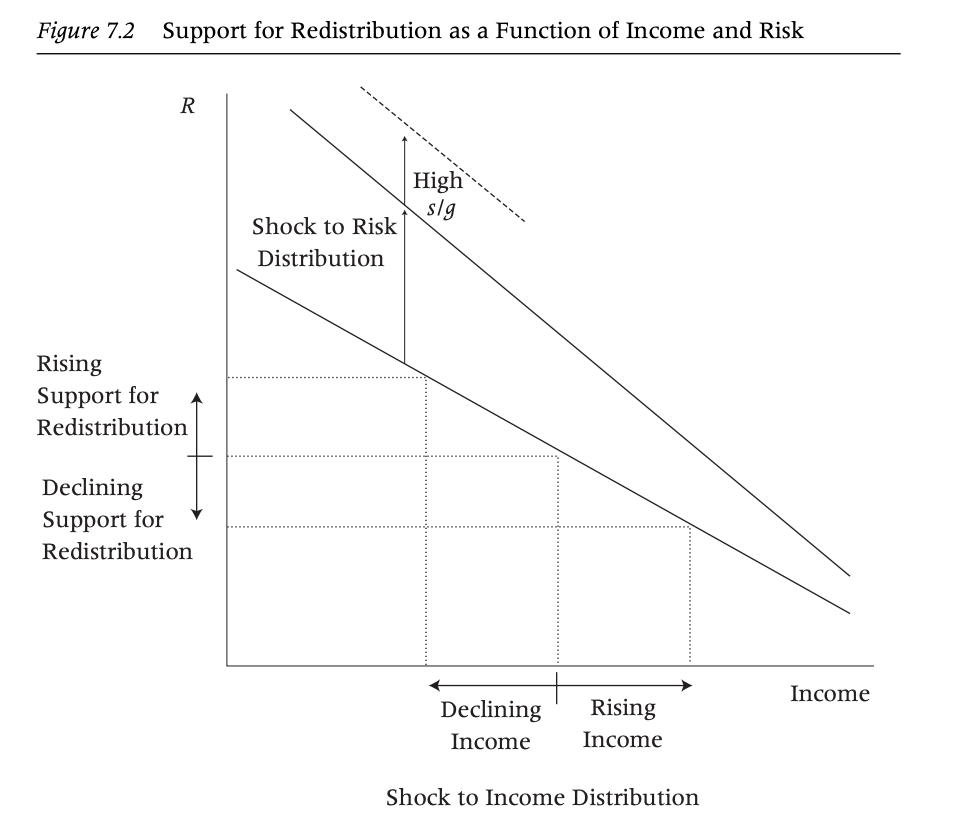
\includegraphics[width=0.6\textwidth]{insurance.png}
\end{frame}
%%%%%%%%%%%%%%%%%%%%%%%%%%%%%%%%%%%%%%%%%%
\begin{frame}{1. The insurance model (Iversen et al.)}
\centering
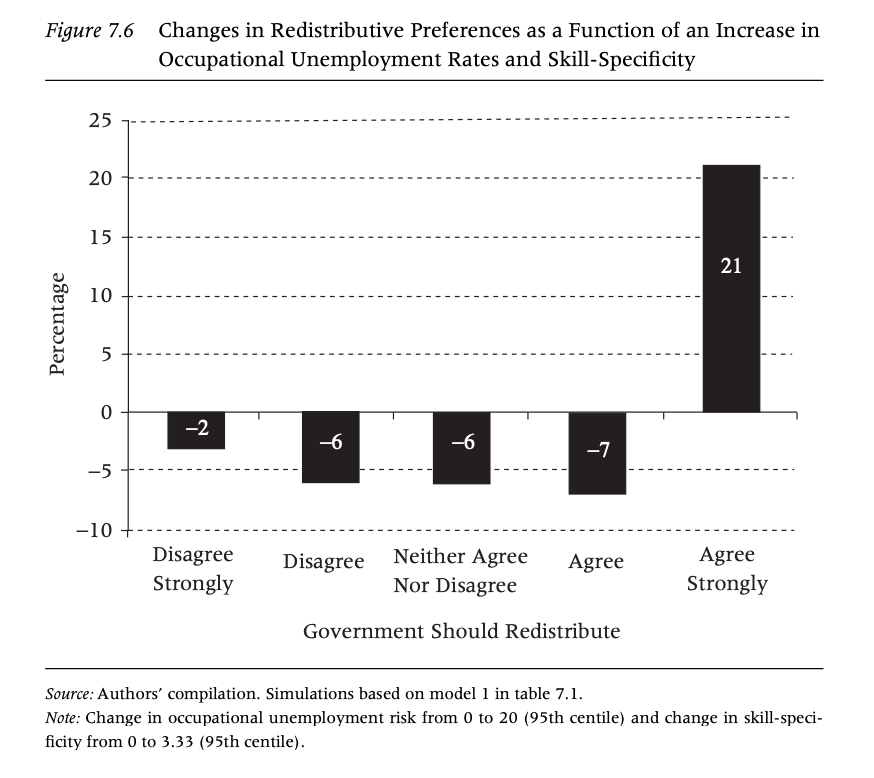
\includegraphics[width=0.7\textwidth]{insurance_2.png}
\end{frame}
%%%%%%%%%%%%%%%%%%%%%%%%%%%%%%%%%%%%%%%%%%
\begin{frame}{1. The insurance model (Iversen et al.)}
\centering
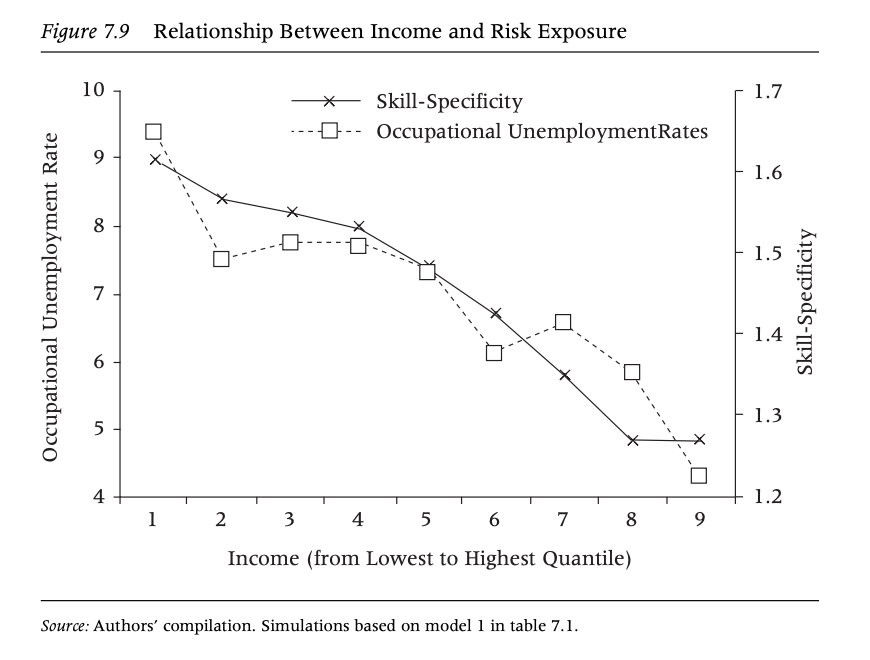
\includegraphics[width=0.7\textwidth]{insurance_3.png}
\end{frame}

%%%%%%%%%%%%%%%%%%%%%%%%%%%%%%%%%%%%%%%%%%
\begin{frame}{2. Non-economic preferences}
\centering
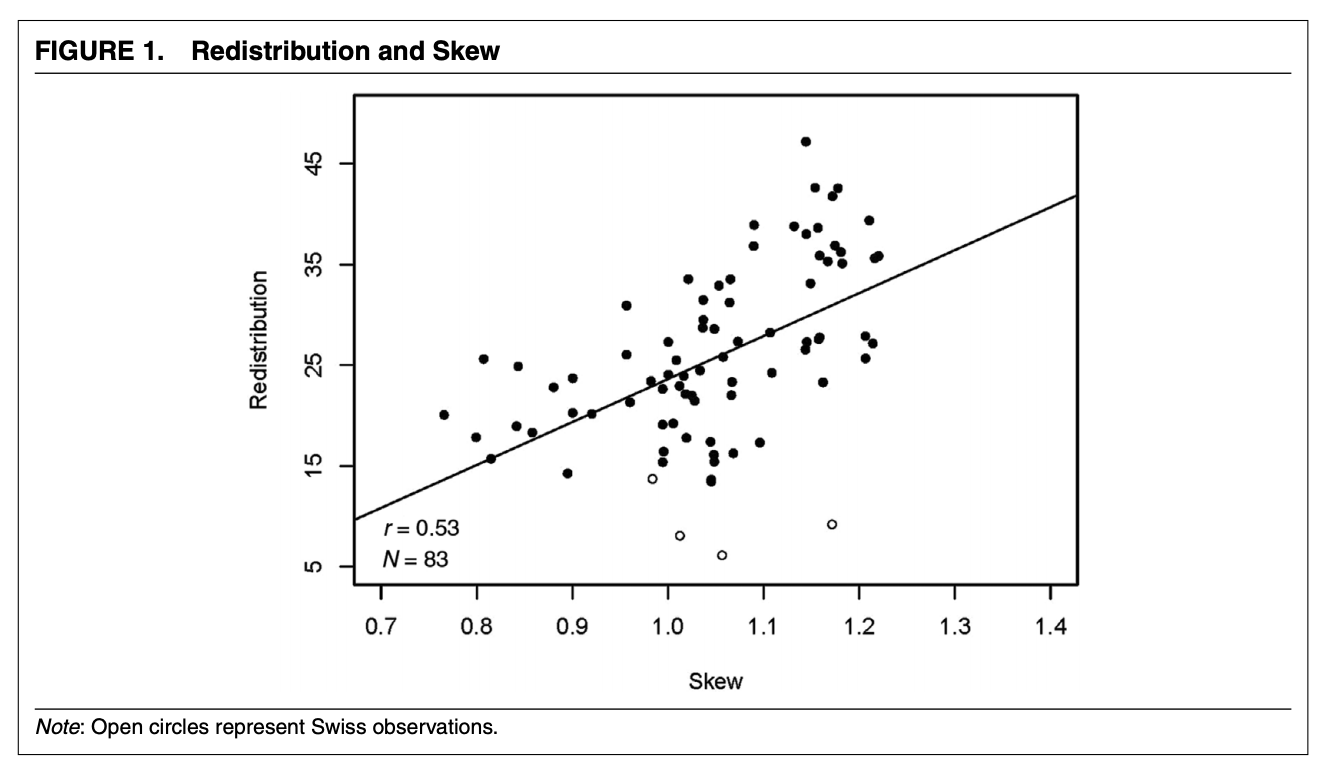
\includegraphics[width=0.7\textwidth]{lupu.png}
\footnotesize \newline  Lupu \& Pontusson, ``The Structure of Inequality and the Politics of Redistribution'', 2011, APSR
\end{frame}

%%%%%%%%%%%%%%%%%%%%%%%%%%%%%%%%%%%%%%%%%%
\begin{frame}{3. Beliefs}
\centering
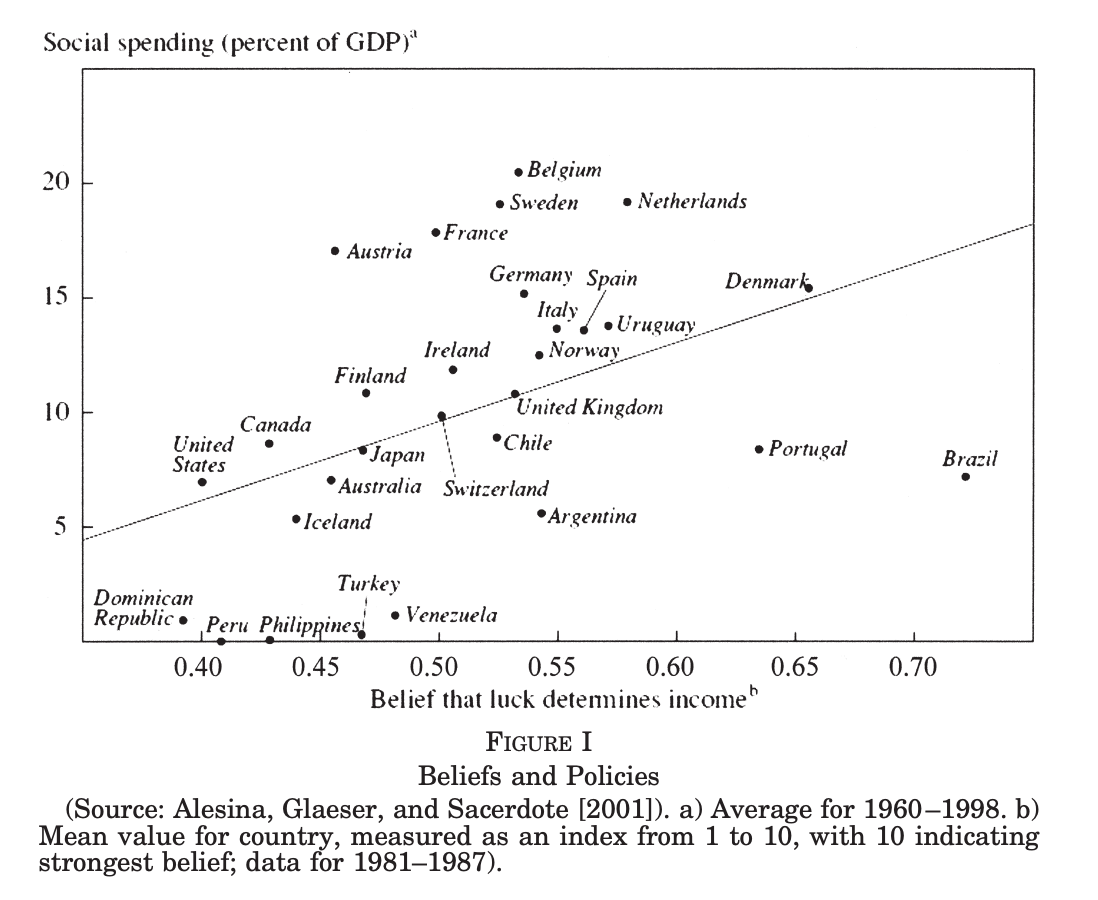
\includegraphics[width=0.65\textwidth]{benabou.png}
\footnotesize \newline  Benabou \& Tirole, ``Belief in a just world and redistributive politics'', 2006, QJE
\end{frame}

%%%%%%%%%%%%%%%%%%%%%%%%%%%%%%%%%%%%%%%%%%
\begin{frame}{4. Issue bundling}
\centering
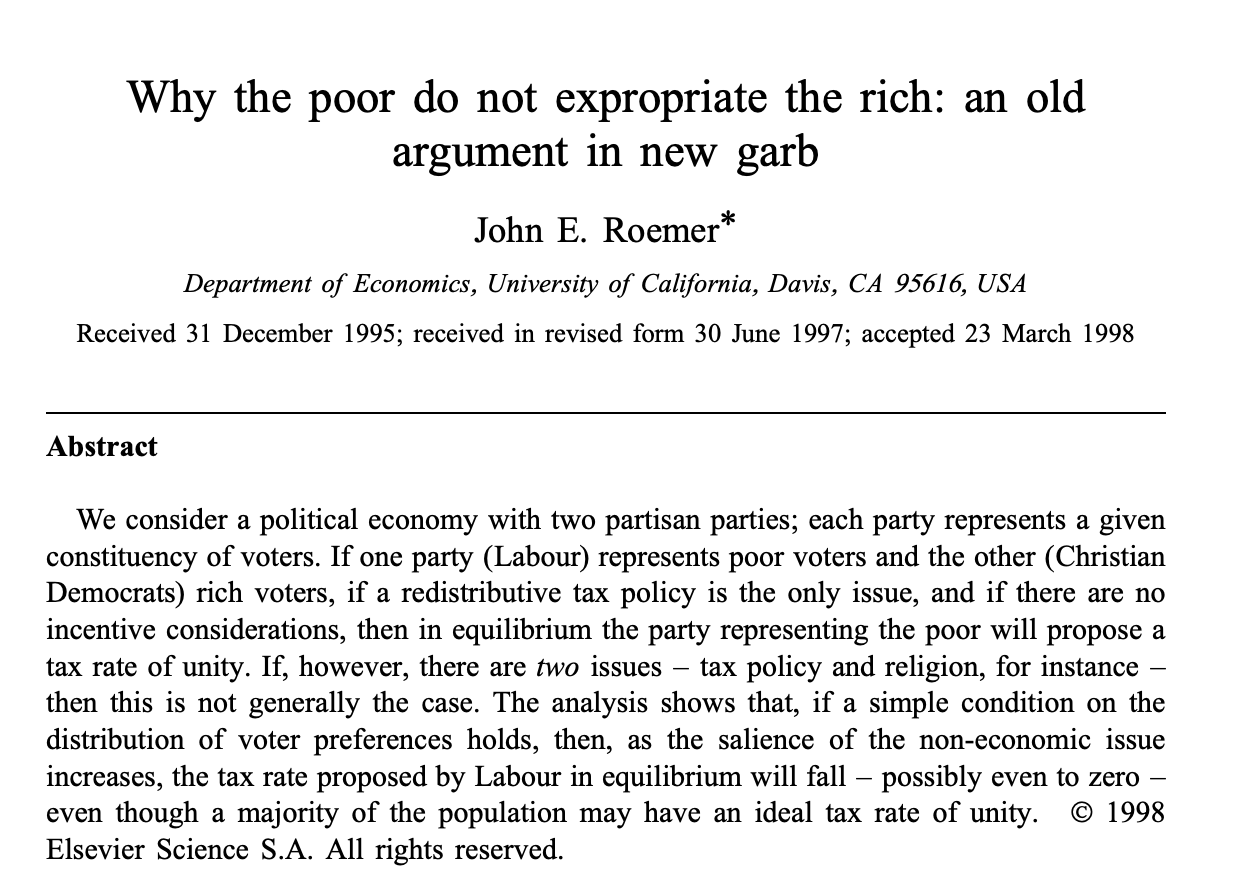
\includegraphics[width=0.65\textwidth]{roemer.png}
\end{frame}



\end{document}